\documentclass[12pt,a4paper]{article}
\usepackage[utf8]{inputenc}
\usepackage{amsmath}
\usepackage{listings}
\usepackage{verbatim}
\usepackage{graphicx} 
\oddsidemargin 0cm
\marginparwidth 0cm
\hoffset 0cm
\usepackage{polski}
\begin{document} 
\large
\begin{tabular}{|c|c|c|c|}
\hline
\multicolumn{4}{|l|}{Temat:}\\
\multicolumn{4}{|c|}{Całkowanie numeryczne metodą Romberga}\\
\hline
\multicolumn{1}{|l}{Wykonał:}&\multicolumn{1}{|l}{Wydział:}&\multicolumn{1}{|c}{Kierunek}&\multicolumn{1}{|l|}{Grupa:}\\
Marcin Fabrykowski&FiIS&Inf. Stos.&grupa 3\\
\hline
\end{tabular}
\normalsize
\vspace{2cm}
\begin{enumerate}
\item Wstęp\\
Metoda Romberga jest rekurencyjną metodą obliczania całek. Polega na tworzeniu tablic całkowych. Tablice te tworzy się na podstawie poniższego algorytmu:
\begin{enumerate}
\item $D_{0,0}=\dfrac{1}{2}\left[f(a)+f(b)\right]$;
\item $D_{n,0}=\dfrac{1}{2}D_{n-1,0}+h_n\sum\limits_{i=1}^{2^{n-1}}f(x+(2i-1)h_n)$
\item $D_{n,k}=\dfrac{4^kD_{n,k-1}-D_{n-1,k-1}}{4^k-1}$
\end{enumerate}
gdzie $h_n=\dfrac{b-a}{2^n}$
\item Wykonanie ćwiczenia\\
Celem ćwiczenia jest wyznaczenie tablic całek dla funkcji
\begin{enumerate}
\item $\int\limits_{-1}^1\dfrac{\sin(x)}{x}dx\ \ ( = 1.892166141)$, dla $n=7$
\item $\int\limits_{0}^\pi\sin(5x)x^2dx\ \ ( = 1.941920881)$, dla $n=10$
\end{enumerate}
Wykresy powyższych funkcji widać na wykresach poniżej.
\begin{figure}
\caption{f1(x)}
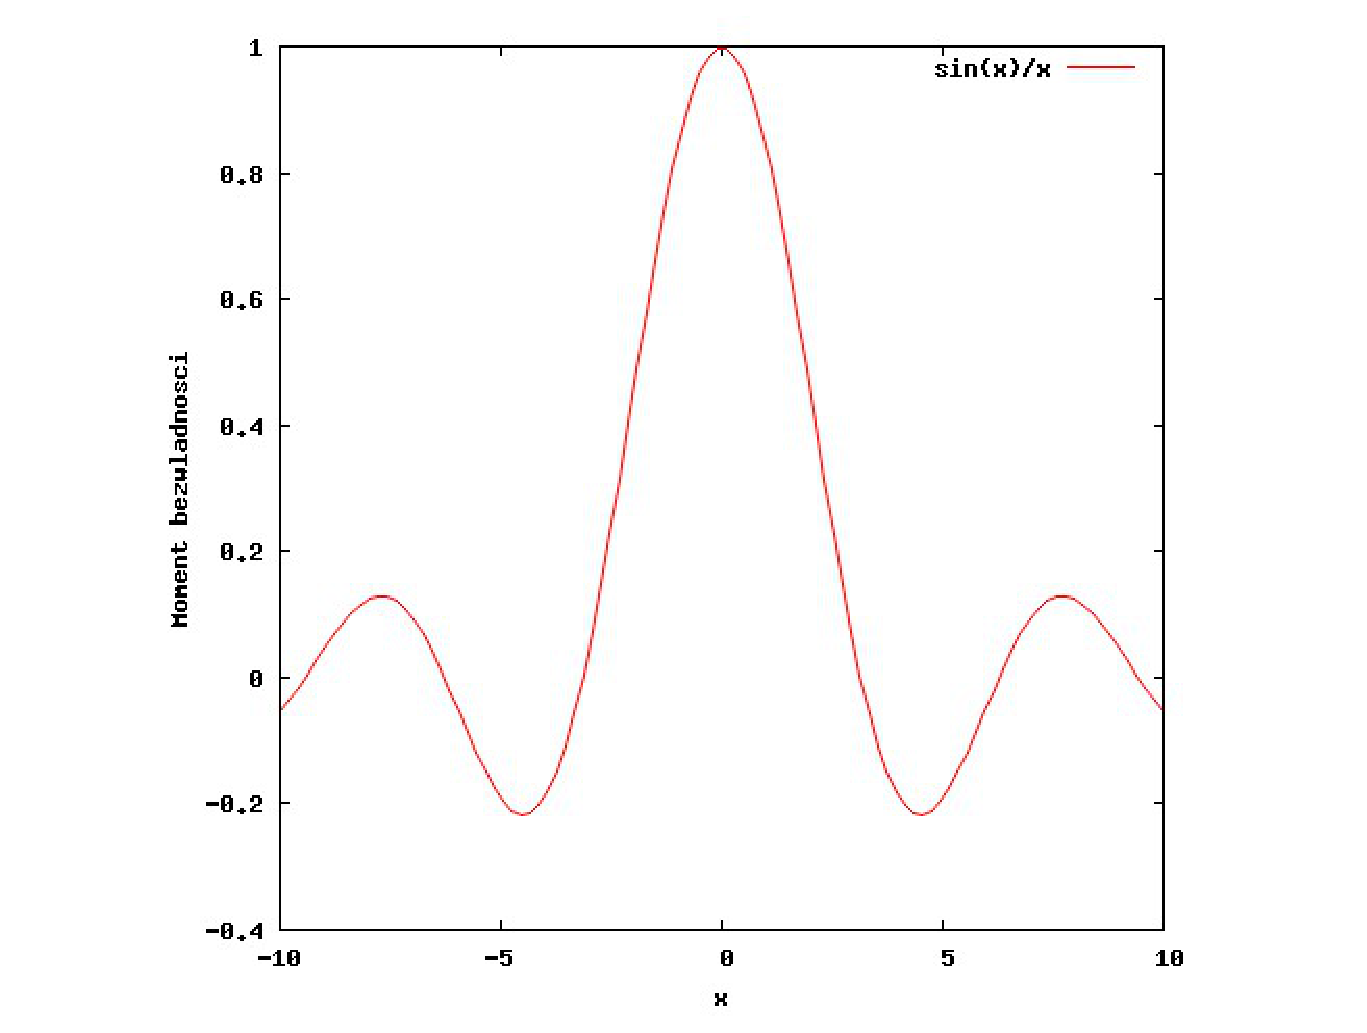
\includegraphics[scale=0.5]{f1.eps}
\end{figure}
\begin{figure}
\caption{f2(x)}
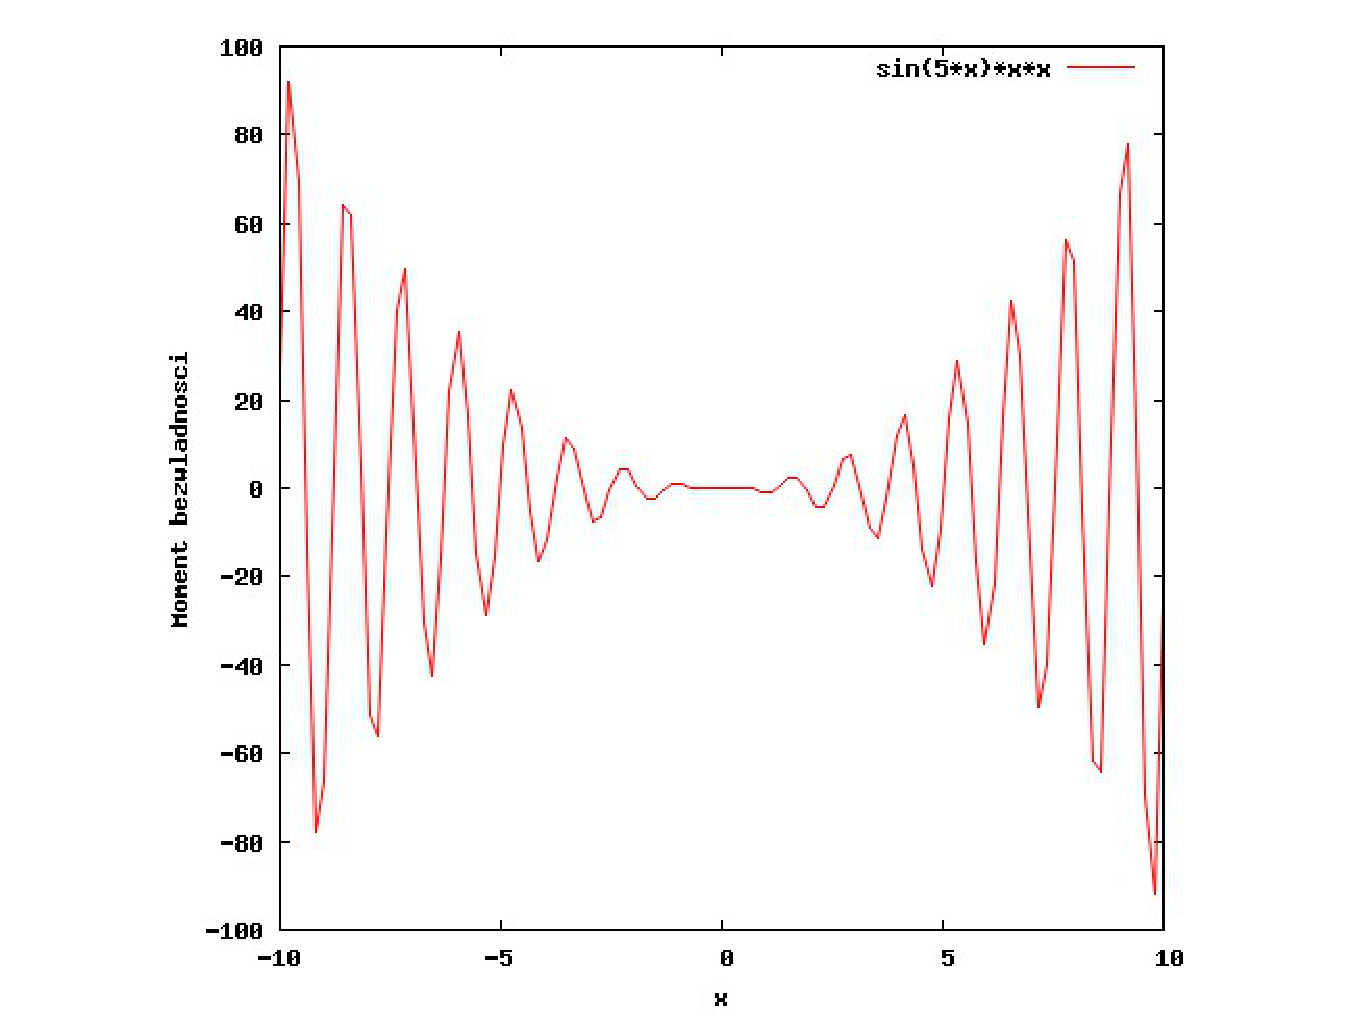
\includegraphics[scale=0.5]{f2.eps}
\end{figure}
Program realizujący powyższe zadanie:
\lstinputlisting[language=C++,caption=main.cpp,breakatwhitespace=true,basicstyle=\footnotesize,breaklines=true,tabsize=4]{main.cpp}
Tabela dla $f1(x)$:
\small
\verbatiminput{f1.dat}
\normalsize
Tabela dla $f2(x)$:
\small
\verbatiminput{f2.dat}
\normalsize
\item Wnioski\\
Można zauważyć, że w~przypadku obu funkcji, wartości na diagonali oraz pierwszej kolumnie dają oczekiwane wartości od 7 iteracji. Wynik jest zadowalający, oraz otrzymany w~krótkim czasie, co pokazuje zasadność używania tej metody.
\end{enumerate}
\end{document}
